%===================================== CHAP 5 =================================


\chapter{Solution Approach} \label{chapter_solution_approach}

The FTCP is a complex problem with a high degree of uncertainty. In each gameweek a large range of decisions must be optimized. Compared to other Fantasy Sports, the gamechips makes it even more complicated. The objective of the model presented in Chapter 4 is to maximize the number of expected points. If the model is run ex-post, expected points equals realized points, and thus the model yields the global optimal solution. However, as stated in the problem description, our aim is to create a model that performs well over an entire season. When competing in Fantasy Premier league, decisions must be made ex-ante. Thus, estimations of expected points and strategies for when the gamechips should be played are required. The aim of this chapter is to provide such input and propose a solution method in order to maximize the performance over the entire season. 

\newpar

In this chapter, the solution approach chosen in order to solve the FTCP is given. The chapter only deals with methodology, real values are not introduced until in Chapter \ref{chapter_experimental_setup}, Experimental Setup. In the first section of this chapter, an overview of the solution method suggested is presented. Next, Section \ref{Forecast_Accuracy} discusses the evaluation of forecasting accuracy. Then, in Section \ref{Player_Performance} methods for predicting player performance are described. Finally, in the Sections \ref{Ch.5_Game_chips} and \ref{Ch.5_Variance_tradeoff} respectively, methods for implementing gamechips and handling risk are proposed.

\begin{comment}
The model presented in Chapter \ref{chapter_model_formulation} fully describes the FTCP. The objective is to maximize expected points over the whole season, assuming a statistical distribution of how many points each player achieves in each gameweek over the entire season. The mathematical model gives the optimal team in each gameweek and the related decisions if it is run ex-post with realized points. Due to the fact that this information is not available ex-ante, it calls for features which predicts future player performance, models the uncertainty and sets a strategy for when the gamechips should be played. Hence, in this chapter we propose a solution method with the aim of achieving highest possible points over a whole season.
\end{comment}
\section{Solution method}

\begin{comment}
In this section a general overview of the different elements in the solution method is explained. Afterwards, in section XX, a more thorough explanation how the solution method operates. 
\end{comment}


\newpar

The solution method is divided in three different elements: player performance prediction, gamechip strategies and risk handling. All the elements can be regarded as input in the model, but in different ways. The predictions are estimations of players' performance and the gamechip strategies are decisions regarding when to play the various gamechips. In order take account for risks such as potential correlation between players on the same or opposing team, additional constraints are introduced. 


\begin{figure}[H]
    \centering
    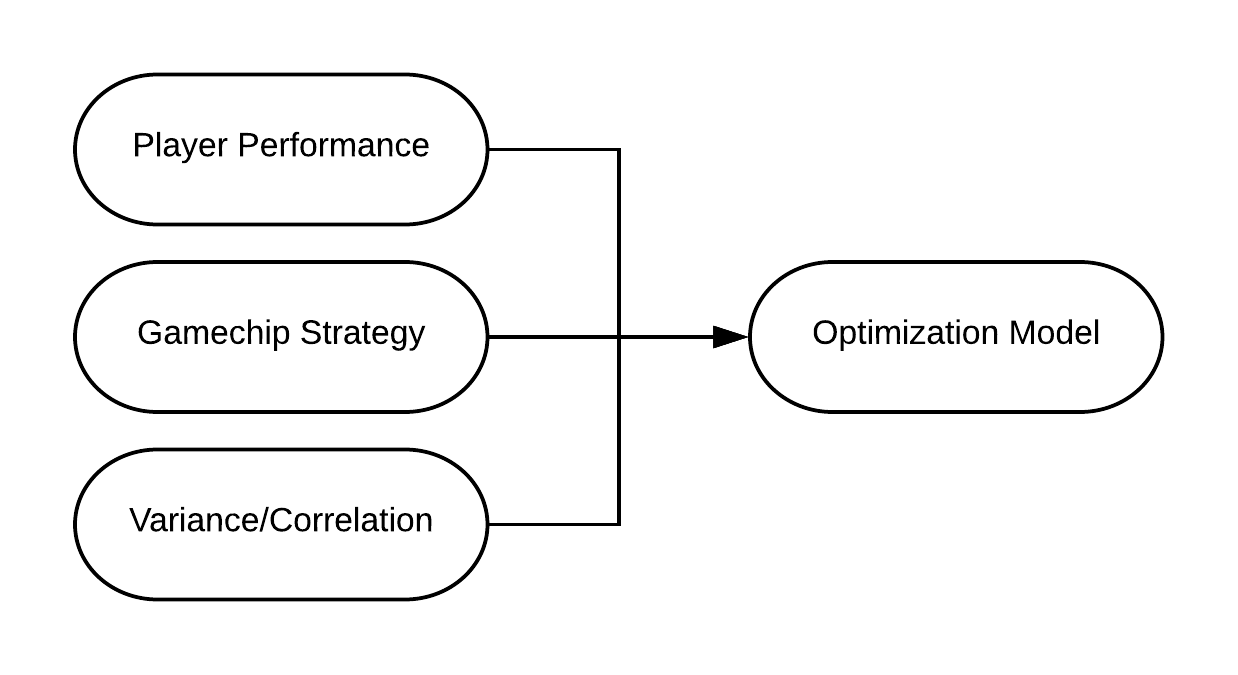
\includegraphics[scale = 0.65]{fig/chapter_5/Solution_Method.png}
    \caption{Elements in the solution method.}
    \label{fig:solution}
\end{figure}

\newpar

In each gameweek the mathematical model is solved for a set of gameweeks and new available information is incorporated. In this thesis, three forecast methods are considered to predict future player performance. The methods are: 
\begin{itemize}
    \item \textbf{Average}. The solution approach suggested by \cite{Bonomo} is adapted and modified to FPL to predict a player's expected points.
    \item \textbf{Regression}. From a pool of explanatory variables related to the FPL, variables are selected and a linear regression model is fitted. 
    \item \textbf{Odds}. Bookmakers' odds can be adjusted to present a probability and consequently are a indicator of future performance of football players. Odds related to scorelines, goals, assists and yellow cards are utilized to estimate expected points. 
\end{itemize}

\newpar

Gamechip strategy are strategies developed to decide when it is optimal to seize the use of gamechips.  There exist limited literature on this topic, henceforth there are a great potential of this implementation. Many interesting approaches could be adopted to decide the optimal use of gamechips, which could either be quantitative or qualitative. The approach adopted in this thesis is to take advantage of future gameweeks which are \textit{blanks} or \textit{double}. The reader is reminded that a blank gameweek is when not all teams play, and a double gameweek is when a team plays more than one match. 

\newpar

As described in Section \ref{Other_Relevant_Research}, there is a large resemblance between the Football Team Composition Problem and the well known Markowitz portfolio selection problem in finance theory. This is taken advantage of and constraints related to handling of risk is incorporated when solving the model. The team's empirical variance and correlation is studied. 


\subsection{Rolling horizon}

The Fantasy Team Composition Problem is solved by a rolling horizon heuristic. The idea behind a rolling horizon heuristic is to split the problem into several sub-problems along a time axis, and then solve them in a chronological order taking into account the solution of the previous sub-problems. The heuristic suits problems with a long planning horizon where there are limited dependency between decisions made early and late in the planning horizon. Industrial planning and scheduling problems are common areas where the heuristic is used. The most important consideration is the number of sub-problems versus the length of each sub-problem. In addition, which decisions to fix in each sub-problem. 

\begin{figure}[H]
    \centering
    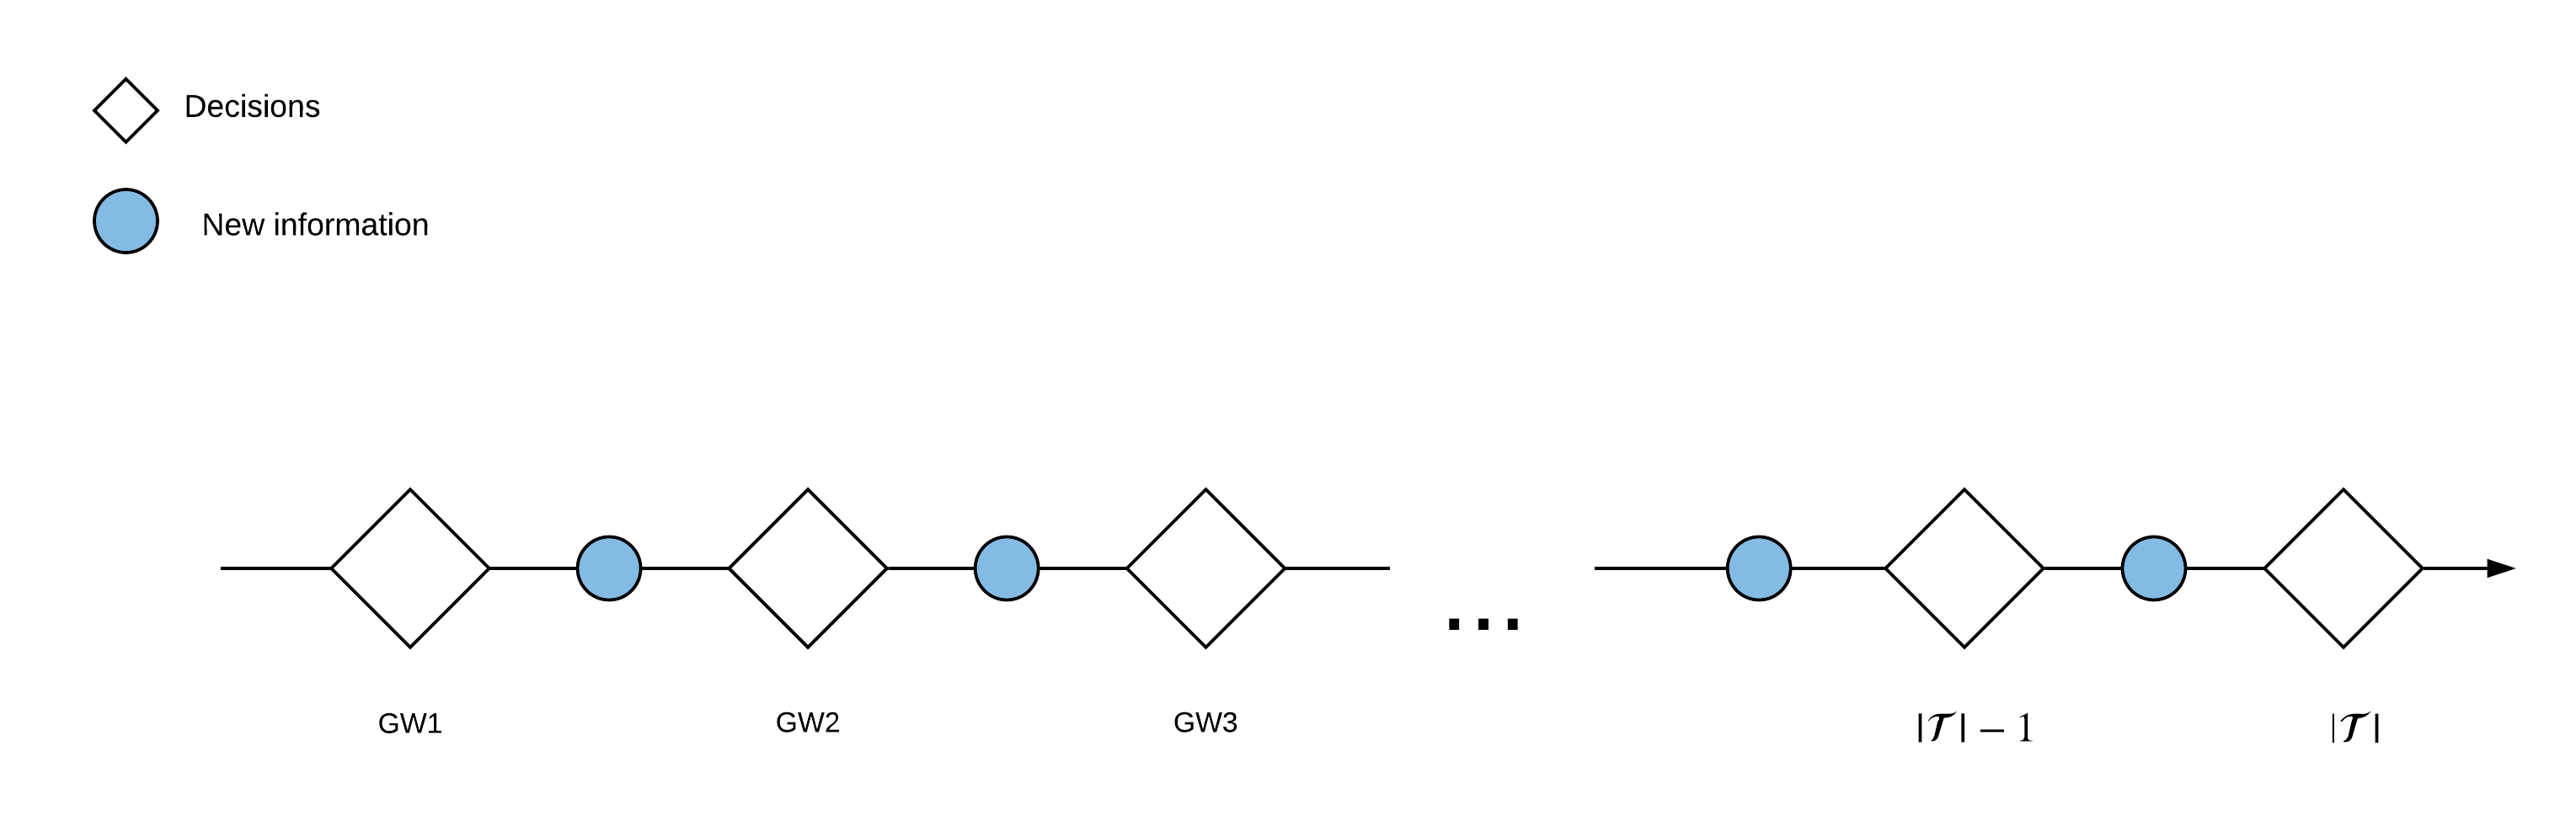
\includegraphics[scale = 0.47]{fig/chapter_5/Rolling_Horizon_Information_Flow.png}
    \caption{Information flow in the FTCP.}
    \label{fig:solution}
\end{figure}

Rolling horizon is an appropriate solution method for FTCP as managers are provided new information and face new decisions every gameweek, i.e. each gameweek is a sub-problem. Consequently, the problem is divided into $\mathcal{T}$ number of sub-problems along a time axis. 

\newpar

The sub-problem is split into three parts:
\begin{itemize}
    \item \textbf{Fixed part (FP)}. Set of gameweeks where decisions have been made and are fixed for the remainder of the solution process. For the FTCP, these decisions are the players that are selected in a gameweek which has to be fixed in the following gameweek. The remaining budget variable, $v$, and the number of free transfers available, $q$, are also fixed in the following gameweek.
    \item \textbf{Central part (CP)}. A gameweek where new decisions are made in the current sub-problem. These are the decisions of which players to add to the selected squad and the starting-lineup, the choice of captain and vice-captain, whether to use a gamechip or not, and which substitution priority to assign. 
    \item \textbf{Predicted part (PP)}. To avoid making too myopic decisions, a predefined number of gameweeks are selected where input data such as expected points, variance and correlation is generated based on information available at that point in time. No decisions are made for these gameweeks. However, the decisions made in CP are based on the prediction in these gameweeks. The FP, CP and PP in a sub-problem are illustrated graphically by figure XX.
\end{itemize}

\newpar

\textit{Here it will be a figure of the difference between FP, CP and FCP and the iterations between them.}

\newpar

The sub-problem is solved for a sub-horizon which in this case is a set of gameweeks. For each iteration, a prediction is made in the PP for how many points each player is expected to attain in the gameweek the CP is in. In addition, predictions are generated for a selected set of following gameweeks. This is modelled into the CP such that it evaluates the impact of future attainable points. In addition, the empirical variance and correlation matrices are calculated and used as input. Before solving for the next sub-horizon, the variable, $x$, for the selected squad in CP is fixed. The remaining budget variable, $v$, and the number of free transfers variable, $q$, are also fixed for the next iteration. These decisions are the decisions that are referred to in the FP. For the next iteration, the gameweek in the previous iteration has been played. The information of the actual scores obtained by each player can now be obtained. 

\newpar

For this problem, the question arises for how many gameweeks the model should look "forward". Specifically, for how many gameweeks should the PP be modelled on, and consequently the decisions made in CP. On one hand, the model should try to optimize for the current gameweek. On the other hand, it should also consider the game fixtures for the next gameweeks. Ideally, this should be tested for several choices of number of gameweeks, in order to see what gives the best result. 


\newpar



\textit{here there will be an algorithm description of we for each gameweek based on new updated information make forecasts, variance and correlation estimation and if the gameweek is a double or blank and henceforth run the optimization model}

\begin{comment}
Any problem with a long planning horizon where there is little
dependency between decisions made early and late in the planning
horizon. Often used in machine scheduling problems, or routing
problems with long planning horizons.

In order to test the mathematical model described in Chapter 4, the model has to be solved for several gameweeks. This is done in manner to examine whether it gives reasonable results. Since big parts of this year’s season has already been played, the mathematical model can be tested in order to see what choices it makes. Hence, it is possible to test its performance. This is done by solving it in a rolling horizon fashion. It is important to emphasize that it is not solved by a rolling horizon method. However, the idea of rolling horizon is implemented in order to see what decisions it makes in the different gameweeks.
The idea is to divide the problem into many sub-problems along a time axis. These are then solved in chronological order, taking into account the solutions of the previous sub- problems.


Having the expected goals appropriately weighted on historic data and the initial probabil- ities of the players’ probabilities of scoring a goal and giving an assist, this information is used to calculate their expected points. Also, by having factors such as yellow cards, red cards and injuries, the degree of complexity increases and the use of simulation is appro- priate. Hence, a simulation is developed in order to forecast a player’s expected points. It is worth mentioning that this could be extended to other approaches such as in a scenario generation, and thus should be regarded as useful. In the next sections, the simulation is explained. First, the simulation is presented generally. Here, the connection between the different parts of the simulation is described. Afterwards, a more thorough explanation of the assigning of goalscorer and assist giver is presented. In the end, the procedure to calculate expected points is described.

\end{comment}


\begin{comment}
- kanskje ha en figur som forklarer hvordan informasjonsflyten er i problemet. 
\end{comment}


\begin{comment}

\begin{enumerate}
    \item \textbf{Player performance prediction}.
    \item \textbf{Gamechip strategy}. 
    \item \textbf{Variance/Correlation}. 
\end{enumerate}

\end{comment}









\begin{comment}
\section{Player performance prediction}\label{Player_performance_prediction}
The optimization model presented in chapter \ref{chapter_model_formulation} uses expected fantasy points as an input. A major uncertainty lies in prediction of football players performances. In this section, we initially present a brief discussion regarding evaluation of forecasting accuracy. Furthermore, we introduce three different methods of predicting future player performance. First, we present a regression model based on the historical Fantasy Premier League performance. Secondly, we replicate and modify the approach suggested by \cite{Bonomo}. Finally, we introduce an approach using bookmakers' odds in order to predict each player's expected points. 
\end{comment}

\newpage

\section{Evaluating forecast accuracy} \label{Forecast_Accuracy}

Before each of the three performance prediction models are introduced in detail, a brief discussion of evaluation of forecasting accuracy is presented.

\subsection{Training and test sets}
In order to determine the accuracy of a forecast, out-of-sample forecasts are evaluated. Available data are separated into two portions: training and test data. A model is first fitted using the training data only. Then, the model's forecast accuracy is determined by comparing forecasts from the model with actual realizations contained in the test data. 
If the model that is the best fit on all available data is chosen as forecasting model, the model would be subject to over-fitting \citep{Hyndman}. That is, the model performs well on the data in the training set, but does not necessarily forecast well.

\subsection{Forecast errors}
A forecast error is the difference between an observed value and its forecast \citep{Hyndman}, as defined as in Equation \ref{eq:f_err}. Here, \{$ y_{1},...,y_{T} $\} is the training set data, \{$ y_{T+1},,y_{T+2},...$\} is the test set data and $\hat{y}_{t+h|T}$ is the forecast at time \textit{T+h}, given \textit{T}. 

\begin{equation}\label{eq:f_err}
    e_{T+h} = y_{T+h} - \hat{y}_{T+h|T}
\end{equation}

\subsection{Scale-dependent errors}

Forecast errors (Equation \ref{eq:f_err}) are on the same scale as the data \citep{Hyndman}. The two most commonly used scale-dependent measures are the MAE (Equation \ref{eq:MAE}) and RMSE (Equation \ref{eq:RMSE}).

\begin{equation}\label{eq:MAE}
    MAE = mean(|e_t|)
\end{equation}

\begin{equation}\label{eq:RMSE}
    RMSE = \sqrt{mean(e_t^2)}
\end{equation}


 A forecast method that minimizes the MAE will lead to forecasts of the median, while minimizing the RMSE will lead to forecasts of the mean \citep{Hyndman}. 
 
\newpage 

\section{Player Performance} \label{Player_Performance}

\textit{Here there will an introduction to this section.}

When using a forecast to estimate the expected value of a player's points, the objective function described in Section \ref{mathematical_model} changes from: 

\begin{equation*}
\smaller
\begin{aligned}
\text{max} \; z ={} & \EX_{\omega} \Big\lbrack\sum\limits_{p \in \mathcal{P}} \sum\limits_{t \in \mathcal{T}} \Big( \mathlarger{\rho}_{pt}(\omega)y_{pt} + \mathlarger{\rho}_{pt}(\omega)f_{pt} + 2 \mathlarger{\rho}_{pt}(\omega)c_{pt} + \epsilon  \mathlarger{\rho}_{pt}(\omega)h_{pt} \\ 
& + \sum_{l \in \mathcal{L}}\sigma_{l} \mathlarger{\rho}_{pt}(\omega)g_{ptl} \Big)  \Big\rbrack \\ 
& - R\sum_{t \in \mathcal{T}}\alpha_{t}
\end{aligned}
\end{equation*}

to 

\begin{equation*}
\smaller
\begin{aligned}
\text{max} \; z ={} &  \sum\limits_{p \in \mathcal{P}} \sum\limits_{t \in \mathcal{T}} \Big( \hat{\mathlarger{\rho}}_{pt} y_{pt} + \hat{\mathlarger{\rho}}_{pt} f_{pt} + 2 \hat{\mathlarger{\rho}}_{pt} c_{pt} + \epsilon  \hat{\mathlarger{\rho}}_{pt} h_{pt} \\ 
& + \sum_{l \in \mathcal{L}}\sigma_{l} \hat{\mathlarger{\rho}}_{pt} g_{ptl} \Big)  \\ 
& - R\sum_{t \in \mathcal{T}}\alpha_{t}
\end{aligned}
\end{equation*}


where $\hat{\rho}_{pt}$ denotes an estimation of expected points of each player $p$ in a gameweek $t$.

\subsection{Player Predictions Using Modified Average}
The solution approach suggested by \cite{Bonomo} can be used for the English Fantasy Premier League as well as for the Argentinian. In general, one simply use the average points performance for the recent gameweeks as the prediction of the performance for the next gameweek. In order to improve the prediction, one can account for team opponent, home advantage and whether a player is on a good performance streak. This is done by weighting a player's performance by three factors as mentioned in section \ref{Forecasting_of_player_performance}.
\newpar
In general, a player's point prediction is calculated according to the following equation:
\begin{equation}
    \textrm{Expected points} = \textrm{Adjusted avg. points} \times \textrm{Team strength} \times \textrm{Home advantage} \times \textrm{Point streak}
\end{equation}
\newpar
Firstly, the solution approach suggested by \cite{Bonomo} is replicated for Fantasy Premier League using their recommended numerical values. Next, we intend to modify and improve the model by using different weights adjusted for historical performance in the English Premier League. Although \cite{Bonomo} uses league table position for measuring the relative strength between adversaries, league position suffers from numerous drawbacks which makes it unreliable for prediction. For example, the league table suffers from high variation in the early stage of the season and low variation in the late stage of the season. Further, competing teams may not share the equivalent number of matches during the season due to postponements, thus providing errors for many rounds. Additionally, the league table does not capture which teams that have faced each other during the season, hence it is inherently biased until the final match of the season has been played. Thus, instead of weighting the teams based on their league position, we utilize an Elo-rating in order to weight the relative team strengths in the league. In addition, an empirical value of home field advantage in the Premier League is used as a factor for the home advantage. In order to measure a player's recent performance, decisions are made on whether a player is on a positive or negative point streak. 
\subsubsection{The Elo system}

The Elo system introduced in section \ref{Strength_of_football_teams} is a rating system used for measuring the relative strength level of sport teams and individual athletes. Within football, the Elo system can be used in order to determine a club's Elo value. The great advantage of the Elo system lies in its simplicity, there is only one value per club at each point in time, the higher the better. 
\newpar
The performance of a team is not measured absolutely; it's inferred from wins, losses and draws against other teams. If team A has a Elo value of $R_A$ and team B has a Elo value of $R_B$, team A has an expected score of 
\begin{equation}\label{eq5.2}
    E_A = \frac{1}{1+10^{\frac{R_B - R_A}{400}}}
\end{equation}
when facing team B. Similarly, team B has an expected score of
\begin{equation}\label{eq5.3}
    E_B = \frac{1}{1+10^{\frac{R_A - R_B}{400}}}
\end{equation}

\newpar
When teams play each other and win or lose, they exchange points. Hence, the club's Elo value is updated once a match has been played. Using the expected scores from equation \ref{eq5.2}, team A's updated Elo value is calculated according to
\begin{equation} \label{eq5.4}
    R^{'}_A = R_A + (S_A-E_A) \times k
\end{equation}
where $S_A$ is the result (1 for win, 0.5 for draw and 0 for loss). Further, $k$ is a factor which determines how fast the Elo value will converge. A higher k-value will have the values converging quicker to their true values, but will suffer from more variation. For smaller k-values, more stable Elo values are created which take longer time to converge. In chess, the World Chess Federation suggest that a value of k=20 should be used for players with an Elo value below 2400. 
\newpar
Similarly, team B's updated Elo value is given by
\begin{equation} \label{eq5.5}
    R^{'}_B = R_B + (S_B-E_B) \times k
\end{equation}
\newpar
In the following, an illustrating example provide how the Elo value of two teams are updated once a match between them has been played:
\newpar
Assume that team A has an Elo value of 1881 and that team B has a value of 1650. If team A faces team B, team A has an expected score according to equation \ref{eq5.2}:
\begin{equation*}
    E_A = \frac{1}{1+10^{\frac{1650-1881}{400}}} = 0.791
\end{equation*}
while team B has an expected score of
\begin{equation*}
    E_B = \frac{1}{1+10^{\frac{1881-1650}{400}}} = 0.209
\end{equation*}
Further, if team A won the match, its Elo value will increase to a value according to equation \ref{eq5.4}: 
\begin{equation*}
   R^{'}_A= 1881 + (1-0.791) \times 20 = 1885
\end{equation*}
As for team B, its Elo value decreases to
\begin{equation*}
   R^{'}_B = 1650 + (0-0.209) \times 20 = 1646 
\end{equation*}

\subsubsection{Using Elo values to rate Premier League teams}
The Elo values provide a sophisticated measurement of the relative strength between the Premier League teams. Further, as the values are updated once a match has been played, the Elo system somehow catches which teams that are in a good form. Elo values can be obtained according to equation \ref{eq5.1} and \ref{eq5.2}. Clubelo.com provide historical Elo values for most of the professional football teams in the world, including teams in the English Premier League, English 1st division etc. These values are used in order to compute the relative team strength in this project, using a k-value of 20. A great advantage of the ratings provided by Clubelo is the fact that these values are modified, taking account for home field advantage, goal difference and inter-league adjustments. In addition, the Elo values from Clubelo incorporates all fixtures and not only league matches.
\newpar
Once the Elo values are obtained, they can be used in order to weight the previous performance of each Fantasy Premier League player. It is likely to suggest that a player playing for a top-rated team has a greater probability of scoring many points than a player playing for a poor team. In addition, a player is more likely to gain many points against a weak opponent than against a top-rated team. Hence, one should consider both the opponent and the team of a player when calculating his previous average. 
\newpar
In table \ref{Elo.1617} some Elo values for the first gameweeks of the English Premier League 2016/17 season are listed. Note that the values are calculated ahead of each gameweek, so that the values in the GW1 column are the Elo values of the teams before gameweek 1 has been played. 

\begin{table}[H]
\centering
\caption{Elo ratings for Premier League 2016/2017}
\label{Elo.1617}
\begin{tabular}{|l|l|l|l|l|l|}
\cline{2-6}
\multicolumn{1}{l|}{} & \multicolumn{1}{l|}{} & \multicolumn{4}{c|}{Elo value}  \\ \cline{2-6} 
\hline
                      & Team                  & GW1    & GW2    & GW3  & GW4    \\
                      \hline
1                     & Chelsea               & 1793   & 1800   & 1798 & 1804   \\
2                     & Tottenham             & 1804   & 1804   & 1800 & 1798   \\
3                     & Man City              & 1848   & 1856   & 1858 & 1863   \\
4                     & Man Utd               & 1789   & 1797   & 1799 & 1804   \\
-                     &                       &        &        &      &        \\
-                     &                       &        &        &      &        \\
-                     &                       &        &        &      &        \\
17                    & Watford               & 1624   & 1631   & 1618 & 1612   \\
18                    & Hull                  & 1589   & 1603   & 1613 & 1608   \\
19                    & Middlesbrough         & 1595   & 1597   & 1601 & 1604   \\
20                    & Sunderland            & 1655   & 1654   & 1636 & 1641   \\
\hline
\end{tabular}
\end{table}

Values from table \ref{Elo.1617} can be used in order to weight the performance of a player. For instance, if a forward received many points against Chelsea, that is more impressive than if the same player equally many points against Sunderland. Hence, one should weight the performances appropriately. In the following, an approach for weighting historical performance is suggested. For instance, let's assume that Paul Pogba, a midfielder at Manchester United received the following points for the first three gameweeks: 


\begin{table}[H]
\centering
\caption{Paul Pogba imaginary points}
\label{my-label}
\begin{tabular}{|l|l|l|l|l|}
\hline
\multicolumn{1}{|c|}{} & \multicolumn{4}{c|}{Points Gained} \\ \hline
Opponent               & GW1        & GW2       & GW3    & GW4   \\
\hline
Chelsea                & 6          &           &        &       \\
Sunderland             &            & 9         &        &       \\
Watford                &            &           & 10     &         \\
Tottenham              &            &           &        & ?      \\
\hline
\end{tabular}
\end{table}

If one simply used his average score for the past three gameweeks in order to predict his performance for the next gameweek, one would predict Pogba to gain 8.33 points in gameweek 4. However, in this case one do not take account for the fact that Manchester United were facing teams of different quality. In addition, one does not consider the fact that Pogba plays for Manchester United, a team that in general performs better than most other teams. As mentioned above, these factors should be considered. Hence, it is necessary to weight the previous performance taking account for the opponent team and the player's team. This can be solved in the following way: 
\newpar
In gameweek 1, Manchester United were facing Chelsea and Pogba earned 6 points. In order to take account for the fact that Pogba plays for Manchester United and were facing Chelsea (a higher ranked team), one simply mulitply his score with Chelseas Elo value and divide it by Manchester Uniteds Elo value. Thus, Paul Pogbas adjusted points should be set to:
\begin{equation*}
    \textrm{Paul Pogba GW1} = 6 \times \frac{1793}{1789} = 6.013 
\end{equation*}
As can be observed, his actual points increases when facing an opponent that is assumed to be better than his team. In contrary, when facing a weaker team, for instance Sunderland his realistic points decreases: 
\begin{equation*}
    \textrm{Paul Pogba GW2} = 9 \times \frac{1654}{1797} = 8.284 
\end{equation*}

In general a players realistic points gained can be calculated by the following equation: 
\begin{equation} \label{actualpoints}
\textrm{Realistic points} = \textrm{Adjusted points} \times \frac{\textrm{Opponent Elo value}}{\textrm{Player's team Elo value}}    
\end{equation}

By calculating realistic points according to equation \ref{actualpoints}, Paul Pogbas adjusted average for the first three gameweeks would be 7.764. The following equation is used in order to calculate the expected points for an upcoming gameweek: 
\begin{equation}
    \textrm{Expected points} = \textrm{Adjusted average} \times \frac{\textrm{Player's team Elo value}}{\textrm{Opponent Elo value}}
\end{equation}
In this way, players are rewarded with an increased expected points when playing for a team with a higher Elo value than its opponent. Hence, his expected performance against Tottenham in the upcoming gameweek 4 would be: 
\begin{equation*}
    \textrm{Expected points for Pogba GW4} = 7.764 \times \frac{1804}{1798} = 7.790
\end{equation*}


\subsubsection{Home field advantage}
As pointed out in section \ref{HomeFieldAdvantage} numerous studies have proven that some kind of home field advantage exist when football games are being played. Football teams have a tendency of performing better when playing at their home field then when playing at their opponents ground. This home field advantage has to be considered when one are to forecast the upcoming performance of the Premier League players. 
\newpar
Usually when one is to determine the home field advantage in a football league, one focuses on the outcome of the game, i.e.  win, draw or loss. In Fantasy Premier League, the outcome of a match has no impact in the point system. As the most important point-factor in FPL is goals scored, the home field advantage has to be calculated in terms of goals. 
\newpar
The home field advantage can be calculated according to the approach suggested by \cite{Pollard}. However, instead of focusing of match outcomes, one determine the advantage by looking into goals. Imagine that each team plays 38 matches during the season, equally divided between home and away games. With 20 teams facing each other twice a season, that implies a total of 380 matches a season. Further, assume that a total of 1000 goals were scored during a particular season. If there were no home field advantage, one would expect that 500 of the goals were scored by the home team and 500 by the away team, yielding a factor of 0.5. However, the results show that 620 of the goals were scored by the home team, which represents 62 \% of the goals scored. With an expected value of 50 \% and an actual value of 62 \% the home field advantage in terms of goals scored can be calculated by: 
\begin{equation*}
    \textrm{Home field advantage} = \frac{\textrm{Actual goals scored home}}{\textrm{Expected goals scored away}} = \frac{0.62}{0.5} = 1.24 
\end{equation*}

Similarly, the away field advantage is calculated according to:
\begin{equation*}
    \textrm{Away field advantage} = \frac{\textrm{Actual goals scored away}}{\textrm{Expected goals scored away}} = \frac{0.38}{0.5} = 0.76
\end{equation*}
\newpar
In this thesis the home field advantage is calculated as an empirical value for the entire Premier League. Hence, each team's home field advantage is not considered. The idea is that the empirical home field advantage along with the relative team strengths calculated by use of the Elo system will give an appropriate representation of a team's performance both home and away. 
\newpar
In order to find an appropriate empirical value for the home field advantage, several previous seasons should be considered. In this project thesis, the empirical value is set to the average of the home field advantage over the past five Premier League seasons. This is due to the fact that the home field advantage value has been stabilized over the past seasons. 

\subsubsection{Player point streak}
Fantasy Premier League managers have a tendency of selecting players that are on a great point streak. As mentioned in section \ref{Forecasting_of_player_performance} \cite{Bonomo} add a factor in order to take account for players point streak. This factor can take a value between 0.95 and 1.05, depending on the duration of a player's point streak. Unfortunately, they do not describe how they determine the value of the point streak factor. Intuitively, the point streak value can be determined in the following way: 
\newpar
If a player receives more than X points 2 gameweeks in a row, his point streak value will be set to 1.01. Further, if the streak continues, the value will increase by 0.01 for each match that his points exceed the X number of points. When a player has received more than X points 6 gameweeks in a row, his point streak value is set to the maximum of 1.05. Hence, the value does not increase if his streak exceeds 6 matches. The same rule applies for players scoring less than Y points 2 gameweeks in a row; then his streak value will be set to 0.99. When scoring less than Y points 6 matches in a row, the point streak value is set to a minimum of 0.95. Once the scoring streak is broken, the player's value is set to 1. 


\subsection{Player prediction using regression}

One way of predicting Fantasy Premier League points is by use of regression. In order to perform a regression and estimate expected points in the next gameweek, numerous numerical and categorical explanatory variables are considered. In the following, all variables considered are presented: 

\newpar

\textbf{Dependent Variable}
\begin{itemize}
    \item A \textbf{realized points} variable can be used as the dependent variable as which the other variables are measured towards. The realized points are the actual points gained by a player for previous gameweeks.
\end{itemize}

\textbf{Independent Variables}

\textit{Categorical Variables}
\newpar
\begin{itemize}
    \item It is reasonable to assume that a player who plays for a good \textbf{team} is expected to gain many points as his team performs well. For instance, defenders playing for teams that does not concede many goals are most likely to keep a clean sheet.
    
    \item The \textbf{position on the field} is worth some attention as well. For instance, it would be interesting to check whether midfielders gain more points than defenders. By figuring out which positions one should focus on, it might be optimal to find an optimal formation for a FPL team.
    \item An important factor is the \textbf{opponent team} a team is facing for a particular gameweek. It is likely that a player gain more points against a rather poor team than a top-ranked team.
    \item Home/Away
\end{itemize}
\newpar

\textit{Numerical Variables}
\newpar
\begin{itemize}
    \item Points in \textbf{previous matches} are incorporated in order to check whether recent performance influence the actual performance of upcoming gameweeks. \item The \textbf{cost} of a player gives an impression of the quality of that particular player. A player listed with a high cost, is expected to gain many points during the season. It would therefore be interesting to check the correlation between a player's cost and his actual point performance.
    \item \textbf{Transfers} made by FPL managers gives one an impression of how other managers expect a player to perform in the future.
    \item Minutes Played
    \item Yellow Cards
    \item Goals Conceded
    \item Saves
    \item Goals
    \item Penalties Missed
    \item Penalties Saved
    \item Clean sheets
    \item Assists
    \item Red Cards
\end{itemize}

\subsubsection{Times Series Effect of points}

It is often argued that form is an important factor in the performance of athletes (kilde). If this is the case, points gained in the closest previous matches could be an interesting exploratory variable. If not, other variables such as total number of goals scored, can be just as predictive. In order to assess if elements of a time series are correlated with each other, \textit{autocorrelation} is a reasonable metric to asses. Just as correlation measures the extent of a linear relationship between two variables, autocorrelation measures the linear relationship between lagged values of a time series \citep{Hyndman}. For example, $r_1$ measures the relationship between $y_t$ and $y_{t-1}$. In general, there exists many autocorrelation coefficients, and the value of $r_k$ can be written as in Equation \ref{eq:rk}. 


\begin{equation}\label{eq:rk}
    r_k = \frac{\sum_{t=k+1}^T(y_t-\bar{y})(y_{t-k}-\bar{y})}{\sum_{t=k+1}^T(y_t-\bar{y})^2}
\end{equation}

The Durbin-Watson test and the Ljung-Box test are two statistical tests one can conduct in order to test for autocorrelation in a time series. The reader is referred to ... for a description of these tests.

\subsubsection{Clustering of Positions}

As points are awarded for different accomplishments for players in different positions, it is likely that different factors play in when predicting their scores. \textit{Here, a rational for the segmentation will be provided}

\subsubsection{Variable selection}

As evident from the previous presentation of (explanatory) variables, a number of such variables are available. If all variables were to be used to build a regression model, the model would very likely be subject to over-fitting \citep{ISLR}. Therefore, in order to limit the number of explanatory variables, a variable selection approach is undertaken. To perform the variable selection, lasso regression is used. In this thesis, only a brief introduction of the concept of lasso regression is given. For a more comprehensive review, the reader is referred to "An Introduction to Statistical Learning" by \cite{ISLR}.\newpar

Lasso regression is a shrinkage method used in order to perform variable selection \citep{ISLR}. The aim is to have the lasso coefficients $\hat{\beta}_{\lambda}^{L}$ minimize the quantity:

\begin{equation*}
    \sum_{i=1}^n\Big (y_i-\beta_0-\sum_{j=1}^p\beta_jx_{ij}\Big)^2 + \lambda \sum_{j=1}^p|\beta_j| = RSS + \lambda \sum_{j=1}^p|\beta_j|
\end{equation*}

Lasso regression penalize the expression one wishes to minimize by absolute value. Or, more precisely, it uses an $l_1$ penalty. This has the desired effect of forcing some of the coefficient estimates to be exactly equal to zero when the tuning parameter $\lambda$ is sufficiently large \citep{ISLR}. Hence, lasso regression performs variable selection.\newpar 

In order to decide the value of $\lambda$, and subsequently what variables to include in the model, a test and a training set is created. Furthermore, different models with different values of $\lambda$ are fitted on the training set. Moreover, predictions based on linear regression for each model associated with a distinct value of $\lambda$ is generated. Finally, the model with lowest RMSE is selected.

\subsubsection{Model Selection}

As the observant reader might have noticed, only one of the exploratory variables presented, namely points in previous matches, is explicitly related to points in previous rounds. This is done in order to limit already complicated dependencies between the exploratory variables. For instance, total points in a season so far would be highly correlated with goals scored so far in a season. Modeling such dependencies, perhaps multiplying the exploratory variables, is a interesting further development. However, is is beyond the scope of this thesis. Instead, we have decided to model the variables deemed significant by the lasso-regression by use of \textit{linear regression}. A linear regression model also has an advantage compared to for instance logistic regressions, as points can be negative.



\subsection{Prediction using odds}
A quite different approach for player point prediction is by use of odds created by bookmakers. It is reasonable to assume that bookmakers provide a realistic odds distribution for the different scorelines, in order to avoid gamblers profiting from an incorrectly odds. By acquiring the result outcomes for each Premier League match, a scoreline prediction can be obtained. By summing all the result odds and dividing each individual result odds by that sum, one can obtain the probability of an exact result to occur. A great drawback with this approach, is the fact that bookmakers only provide odds for the upcoming gameweek. Hence, the odds can only be used in order to predict the fantasy points one gameweek ahead. 
\newpar
When the scoreline predictions are acquired by use of result odds, one has to link these predictions to player performances. In order to determine the probability for a defender or midfielder to keep a clean sheet, one simply sum the probabilities of each match outcome where its team does not concede a goal. Further, bookmakers provide odds' for each individual player to score a goal or have an assist in a particular match. By summing the goalscorers odds, one can obtain the cumulative probability distribution of the goalscorers. Once the cumulative distribution is obtained, one simply multiply the goalscoring probabilities with the result probabilities in order to assign goalscoring points for each player. As for the assist, a similar approach may be used. However, some of the goals scored are unassisted which must be taken account for when predicting the assist points. This can be done by multiplying a players assist points with a factor representing the amount of goals being assisted. Finally, as for the yellow cards, one simply use the odds in order to calculate the probability of a player receiving a yellow card. For instance, if a player has a probability of 0.3 for receiving a yellow card in a particular match, his expected points is penalized with -0.3 as a yellow card deducts 1 point. 
\newpar
The largest bookmaking companies offers odds for all the items mentioned in the paragraph above. As goals scored are the greatest point factor in Fantasy Premier League, this area is of great interest. As mentioned, it is necessary to to obtain the probabilities for each result outcome in a given match. The following example provides Unibet's result odds for a match-up between Leicester and Burnley on April 14th 2018. 

\begin{table}[H]
\centering
\caption{Result odds for Leicester-Burnley 14.04.18}
\label{Leicester-Burnley}
\begin{tabular}{|ll|ll|ll|}
\multicolumn{6}{c}{Odds}                   \\
\hline
1-0 & 7.00   & 0-0 & 7.50   & 0-1 & 8.00   \\
2-0 & 11.00  & 1-1 & 6.00   & 0-2 & 13.00  \\
2-1 & 9.50   & 2-2 & 15.00  & 1-2 & 10.50  \\
3-0 & 23.00  & 3-3 & 67.00  & 0-3 & 29.00  \\
3-1 & 21.00  & 4-4 & 301.00 & 1-3 & 23.00  \\
3-2 & 31.00  &     &        & 2-3 & 35.00  \\
4-0 & 61.00  &     &        & 0-4 & 81.00  \\
4-1 & 56.00  &     &        & 1-4 & 67.00  \\
4-2 & 81.00  &     &        & 2-4 & 91.00  \\
4-3 & 181.00 &     &        & 3-4 & 201.00 \\
5-0 & 201.00 &     &        & 0-5 & 276.00 \\
5-1 & 181.00 &     &        & 1-5 & 226.00 \\
5-2 & 276.00 &     &        &     &        \\
\hline
\end{tabular}
\end{table}

The odds provided in table \ref{Leicester-Burnley} can be translated into match result probabilities. This is done by summing all the inverse odds and afterwards dividing each inverse odds by the sum. The results are shown in table \ref{Prob.Lei-Bur}.


\begin{table}[H]
\centering
\caption{Probabilities for Leicester-Burnley 14.04.18}
\label{Prob.Lei-Bur}
\begin{tabular}{|ll|ll|ll|}
\multicolumn{6}{c}{Odds}                         \\
\hline
1-0 & 0.104388 & 0-0 & 0.097429 & 0-1 & 0.09134  \\
2-0 & 0.066429 & 1-1 & 0.121786 & 0-2 & 0.056209 \\
2-1 & 0.076918 & 2-2 & 0.048714 & 1-2 & 0.069592 \\
3-0 & 0.03177  & 3-3 & 0.010906 & 0-3 & 0.025197 \\
3-1 & 0.034796 & 4-4 & 0.002428 & 1-3 & 0.03177  \\
3-2 & 0.023571 &     &          & 2-3 & 0.020878 \\
4-0 & 0.011979 &     &          & 0-4 & 0.009021 \\
4-1 & 0.013049 &     &          & 1-4 & 0.010906 \\
4-2 & 0.009021 &     &          & 2-4 & 0.00803  \\
4-3 & 0.004037 &     &          & 3-4 & 0.003635 \\
5-0 & 0.003635 &     &          & 0-5 & 0.002648 \\
5-1 & 0.004037 &     &          & 1-5 & 0.003233 \\
5-2 & 0.002648 &     &          &     &         \\
\hline
\end{tabular}
\end{table}

Once these probabilities are obtained, it is possible to calculate the expected goals scored by Leicester. This is done by multiplying the probability of a result occuring by the amount of goals scored by Leicester in that particular result. Further, one have to sum all the probabilities in order to find Leicester's expected goals scored. In the example from table \ref{Prob.Lei-Bur} Leicester's expected goals is found to be 1.234. 
\newpar
Further, it is necessary to assign expected goalscoring- and assist points to each player. For instance, if Jamie Vardy has a cumulative probability of 0.26 of scoring a goal for Leicester, his expected goalscoring odds is found by multiplying 0.26 with the expected goals scored by Leicester. 
\begin{equation*}
    \textrm{Jamie Vardy expected goals scored} = 1.234 \times 0.26 = 0.321
\end{equation*}

Finally, his expected points gained from scoring goals is calculated according to the Fantasy Premier League point system: 

\begin{equation*}
    \textrm{Goal points Jamie Vardy} = 0.321 \times \textrm{4 points} = \textrm{1.284 points}
\end{equation*}

A similar approach can be used in order to calculate a player's expected points from assists. However, one have to consider the fact that not all goals are assisted: 

\begin{equation*}
    \textrm{Expected assist points} = \textrm{Expected goals} \times \textrm{Player's assist probability} \times \textrm{Assist probability}
\end{equation*}

As for the clean sheets, the probability of a team keeping a clean sheet is found by summing the probabilities of all the result outcomes were the team does not concede a goal. According to table \ref{Prob.Lei-Bur} Leicester has got a probability of 0.316 for keeping a clean sheet. Hence, the starting defenders and the  goalkeeper are expected to gain

\begin{equation*}
    0.316 \times \textrm{4 points} = \textrm{1.264 points}
\end{equation*}
from keeping a clean sheet. 

\newpar
In addition, one can use odds for yellow cards in order to calculate a player's expected deducted points for receiving a yellow card. On the bookings sites each player is listed with an odds for a probability of being booked. The probability of receiving a yellow card is simply the inverse of the odds. For instance, if a player is listed with an odds of 3.00 for receiving a yellow card, it is a probability of

\begin{equation*}
    \frac{1}{3.00} = 0.333 
\end{equation*}

that the player receives a yellow card. Hence, his expected points is deducted with:

\begin{equation*}
    0.333 \times \textrm{1 point} = \textrm{0.333 points.} 
\end{equation*}

\begin{comment}
Kanskje skrive noe om format og behandling av dataen. Dette gjøres når all data fra Sportradar er på plass...
\end{comment}


\newpage
\section{Gamechips}\label{Ch.5_Game_chips}
In the following we present how the game chips are implemented in the model. Human FPL managers have to make decisions of when to use their gamechips, i.e. they have to decide whether it is best to play them in a given gameweek or if it is optimal to wait. As the model is solved using a rolling horizon approach, a strategy for when to use the gamechips is required. Many different approaches can be undertaken in order to develop such a strategy. The model is solved over a sub-horizon, so there is nothing that prevents the model from not using the gamechips in the current sub-problem. Therefore, an interesting approach would be to consider a type of punishment in terms of points for the use of gamechips. Another interesting approach would be to model use of gamechips analogous to how a financial option is valued. A third option is to base the decisions on intuition. We have decided to undertake the latter approach. A lot of theories have emerged on when it is optimal to use the chips (kilder). Regardless, more quantitative approaches have huge potential and are exciting topics for future research.

\newpar
The first wildcard, which has to be played within the first half of the season, is usually played at the end of the first quarter of the season. Human managers often use the wildcard in the region between gameweek 8 and gameweek 12. The model is given the opportunity to play a wildcard in one particular gameweek, where it can either choose to play it or to disregard it for the first half of the season. 
\newpar
As for the triple captain, it is wise to played it in a double gameweek as players are expected to gain more points when featured twice. Thus, the model is given the opportunity to play the triple captain in the first double gameweek of the season. 
\newpar
The second wildcard should be played with caution, as it is wise to also consider the bench boost chip when using it. As the bench boost allows each player in the squad to collect points, and not only the starting lineup, the bench boost should be played in a double gameweek. Therefore, the model is set to play the second wildcard in the gameweek ahead of a double gameweek.
\newpar
Finally, the free hit, which allows the manager to perform unlimited free transfers for one gameweek, should be used wisely. There are in general two cases were playing the free hit is reasonable. First, the free hit could be played in a blank gameweek, i.e. a gameweek consisting of less than 10 fixtures. This is done to ensure that all the players in your starting lineup are featured for that particular gameweek. Another wise choice is to play the free hit in a double gameweek, ensuring that the majority of your starting lineup consists of players that are featured twice. 





\newpage
\section{Expected Points/Variance trade-off} \label{Ch.5_Variance_tradeoff}

In the literature review, it is pointed out that the FTCP has a lot of similarities with portfolio optimization. In financial optimization it is common to examine the expected return/variance trade-off \citep{Markowitz}. According to \cite{Zenios}, the variance of a portfolio of \textit{n} assets with weight \textit{w} can be expressed as 

\begin{equation}
    \sigma^2(w) = \sum_{i = 1}^{n}\sum_{i' = 1}^{m}\sigma_{ii'}w_iw_{i'} = \sum_{i = 1}^{n}\sigma_{i}^2w_i^2 + \sum_{i = 1}^{n}\sum_{\substack{i' = 1;\\ i' \neq i}}^{n}\sigma_{ii'}w_iw_{i'}
    \label{eq:port_var}
\end{equation}

where, $w_i$ is the portfolio weight of asset $i$, $\sigma_{i}^2$ is the variance of asset \textit{i} and $\sigma_{ii'}$ is the covariance between assets $i$ and $j$. \newpar

In our case, we can rewrite Equation \ref{eq:port_var} by utilizing the fact that each portfolio weight is either $\frac{1}{11}$ or $0$. If we also substitute the expression for covariance with correlation, the expression simplifies to

\begin{equation}
    \sigma^2(y) = (\frac{1}{11})^2\sum_{i = 1}^{n}\sigma_i^2y_i + (\frac{1}{11})^2\sum_{i = 1}^{n}\sum_{\substack{i' = 1;\\ i' \neq i}}^{n} \sigma_i^2\sigma_j^2y_iy_j\rho_{i,j}
    \label{eq:team_var}
\end{equation}

where $\sigma_{i}^2$ is the variance of expected points obtained by player \textit{i}, $\sigma_{j}^2$ is the variance of expected points obtained by player \textit{j} and $\rho_{i,j}$ is the correlation between expected points obtained by player $i$ and player $j$. In addition, $y_i$ and $y_j$ are binary variables indicating whether player $i$ and player $j$ is included in the starting team (portfolio) of players.\newline

In the optimization, we now may determine an upper threshold for the variance of the team at time $t$ as described below. Note that in Equation \ref{eq:team_var} two binary variables are multiplied. In order to linearize the expression, the following set of equations are inferred.

\begin{equation}
    \sigma^2_{t} = (\frac{1}{11})^2\sum_{p = 1}^{P}\sigma_p^2 y_{pt} + (\frac{1}{11})^2\sum_{p = 1}^{P}\sum_{p' = 1}^{P} \sigma_p^2\sigma_p'^2\rho_{p,p',t} \delta_{pp't} \qquad\qquad t \in \mathcal{T}
\end{equation}

\begin{equation}
    \sigma^2_{t} \leq THRESHOLD \qquad\qquad t \in \mathcal{T}
\end{equation}

\begin{equation}
    \delta_{pp't} \leq y_{pt}  \qquad\qquad p \in \mathcal{P}, p' \in \mathcal{P}, \enskip t \in \mathcal{T}
\end{equation}

\begin{equation}
    \delta_{pp't} \leq y_{p't}  \qquad\qquad p \in \mathcal{P}, p' \in \mathcal{P}, \enskip t \in \mathcal{T}
\end{equation}

\begin{equation}
    \delta_{pp't} \geq y_{pt} + y_{p't} - 1  \qquad\qquad p \in \mathcal{P}, p' \in \mathcal{P}, \enskip t \in \mathcal{T}
\end{equation}



\subsection{Variance}
By variance, the variability in each players performance (points obtained) is meant. Some midfielders are known to be consistently starting, but seldom contribute in terms of assists or goals. Such players probably have a low expected value of points, but also a low variability in points earned. Other players might contribute a lot in terms of assists and goals when they are playing, but are perhaps often injured. Such players could have a high predicted value, but also a high variance in points obtained.\newpar

\subsection{Correlation}
The variance of each player only considers each player's individual contribution to the team's total variance. However, it is natural to assume that there exists a correlation between the performance of players. For instance, as both a goalkeeper and defenders of the same team points for keeping a clean sheet, their performances are expected to be positively correlated. Similarly, it is intuitive that the goalkeeper and forwards of two opposing teams are negatively correlated. Whether or not there exists correlation between defenders of opposing teams are perhaps not so obvious. \newpar

\begin{comment}
\subsection{Further discussion}
\begin{itemize}
    \item Na = average (bare aktuelt når spilleren kun har spilt en kamp, før det vil han ikke velges) 
    \item 0 = min $>$ 0
    \item tar med alle tilgjengelige observasjoner
    \item diskutere om fordeling
    \item varians eller standardavvik
    \item only non-zero data considered
    \item what hypotesis test is performed
\end{itemize}
\end{comment}











